\section{Complete physical model}\label{sec:et:coupling}
To model the fluid motion of a charged fluid under influences of
electrostatic forces, a coupling between different models is
considered.

The electric field and potential in the system are obtained from
solving Poisson's equation for electrostatics (section
\ref{sec:et:poisson}) with a given charge density. This Charge density
is obtained from the Nernst-Planck equation (section
\ref{sec:et:np}) by including effects on
the charge distribution from the electric field previously mentioned,
diffusion and advection. The advective charge flux is given from the
velocity field in the fluid that is obtatined by solving the
Navier-Stokes equations (section
\ref{sec:et:ns}). Forces due to present electric fields on net
charged areas of the fluid also couples the NS equations to the NP
equation. More about the force coupling is discussed in
sections. \ref{sec:et:streaming_pot} and
\ref{sec:et:electroosmosis}. The coupling between the different
equations are visualised in fig. \ref{fig:coupling}.

\begin{figure}
\begin{center}
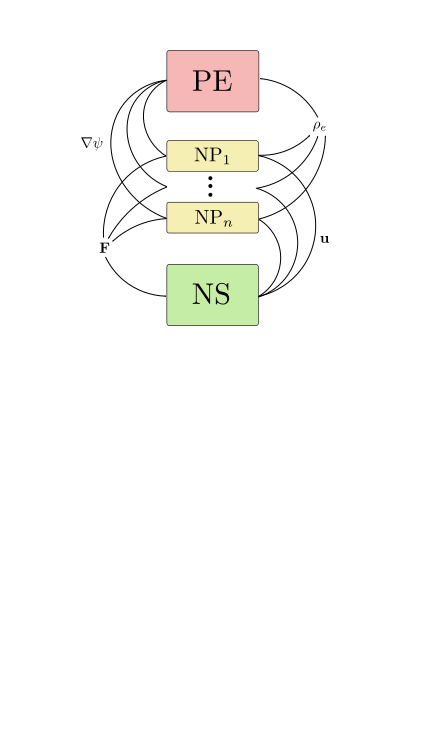
\includegraphics[width=0.5\textwidth]{fig/coupling.pdf}
\end{center}
\caption{Visualisation of the coupling between the three equations
  present in the model. Poisson's equation (PE), The set of
  Nernst-Planck equations (NP$_1$ ... NP$_n$) and the Navier-Stokes
  equations (NS). The dependencies have also be marked with arrows
  indicating what quantities for a certain equation that are needed
  from an other.}
\label{fig:coupling}
\end{figure}

%The algorithm to solve the coupled equations is described in section
%\ref{lb:algorithm}.

